\documentclass{beamer}
\graphicspath{{./Figures/}}   
\usepackage{b2latex}
\usepackage{bsymb}
\usepackage{listings}
\usepackage{subfigure}
\usepackage[utf8x]{inputenc}
\usepackage{default}
\usetheme{Madrid}
\title{The Theory Plug-in: a tutorial} 
\subtitle{Presented by Andy Edmunds}
\author[I. Maamria]{Issam Maamria}
\institute{University of Southampton}
%\date{March 27th, 2012}

\begin{document}
\maketitle

\begin{frame} 
\frametitle{Outline}
\tableofcontents
\end{frame} 

\section{Motivation}
	\begin{frame}
		\frametitle{Motivation}
		\begin{enumerate}
			\item Provide a mechanism to extend the mathematical language.

~

			\item Provide a mechanism to extend the proof infrastructure.

~
			\item Ensure that both mechanisms do not compromise soundness of the formalism.

~
			\item Relieve the end-user from having to write code for simple extensions.

~
			\item Ensure practicality and ease of use in any resultant tools.
		\end{enumerate}
	\end{frame}

\section{The Theory Plug-in}
	\begin{frame}
		\frametitle{The Theory Plug-in $\rightarrow$ Mathematical Extensions}
\begin{center}
\begin{minipage}[t]{0.5\textwidth}
		A theory can define:	

~	

		\begin{itemize}
			\item Datatypes,

~

			\item Operators, 


~
			\item Polymorphic theorems, 

~
			\item Rewrite and inference rules.
		\end{itemize}
\end{minipage}
\end{center}
	\end{frame}

	\subsection{Capabilities}
	\begin{frame}
		\frametitle{The Theory Plug-in $\rightarrow$ Capabilities}
		\begin{itemize}
			\item A theory component is the place holder for defining new `extensions'.

~

			\item Theories are polymorphic on the type parameters which they define.

~
			\item Theories are subject to static checking and proof obligation generation.

~
			\item Proof obligations generated from theories aim to ensure soundness is not compromised.
		\end{itemize}
	\end{frame}
	\begin{frame}
		\frametitle{The Theory Plug-in $\rightarrow$ Capabilities}
		\begin{itemize}
			\item Theory \emph{Deployment} takes theories from `development mode' to `production mode'.

~

			\item At this stage users should have discharged all proof obligations that have been generated by the theory plug-in.

~
			\item IMPORT establishes a partial order between theories.

~
			\item Once a theory is deployed, no further work is required from the user. Extensions are immediately usable in models and proofs.

~

			\item The plug-in does all the work related to: polymorphism/pattern matching, type checking, well-definedness ...
		\end{itemize}
	\end{frame}

\section{The Theory Component}
	\begin{frame}
		\frametitle{The Theory Component}
		\begin{figure}
			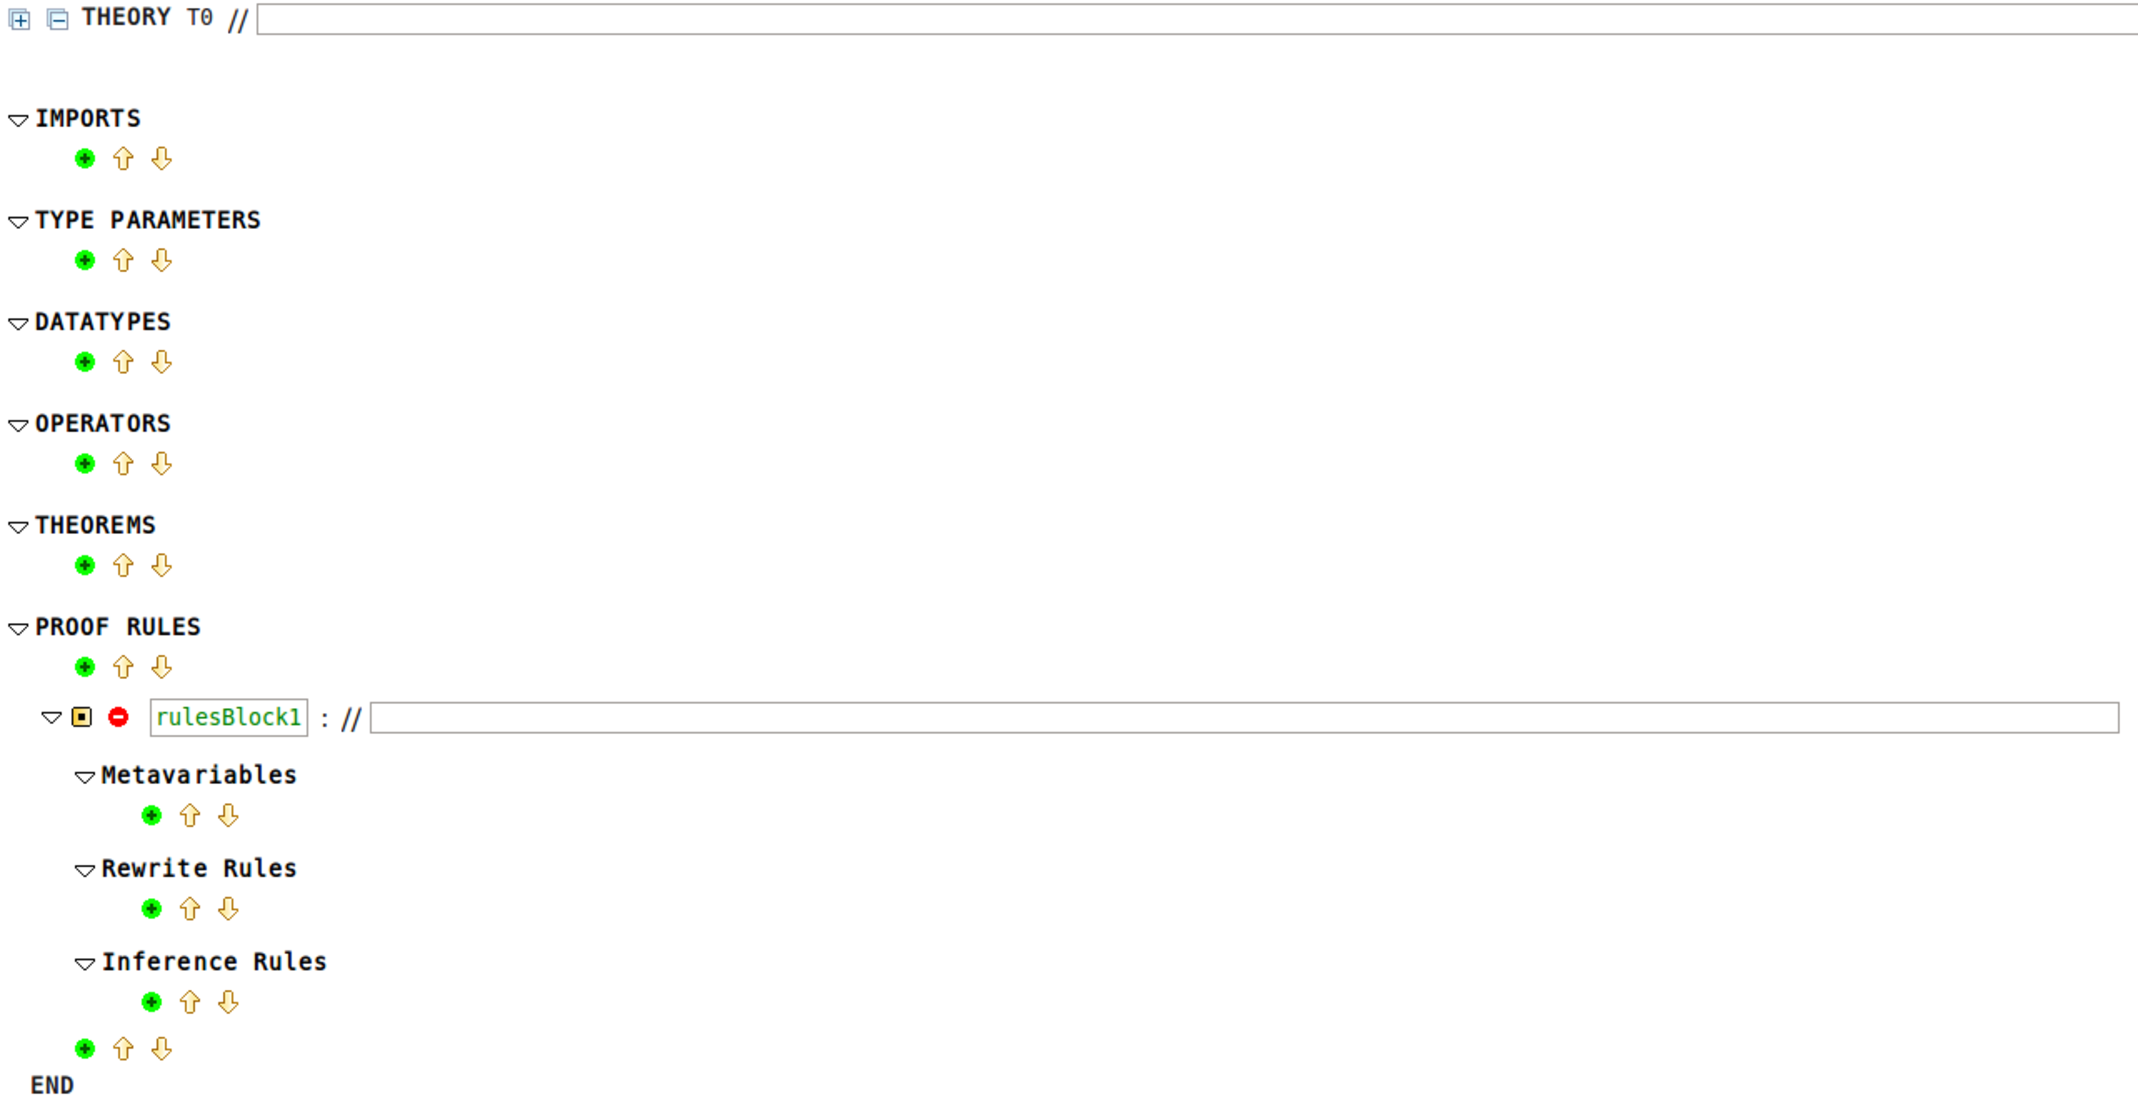
\includegraphics[scale=0.3]{Theory}
		\end{figure}
		\begin{itemize}
			\item We will explain each sub-element of the theory.
		\end{itemize}
	\end{frame}
	\begin{frame}
		\frametitle{The Theory Component}
		\begin{itemize}
			\item Machines and Contexts \emph{Use} Theory Components
			\begin{itemize}
				\item But, there is no explicit `uses' clause.
			\end{itemize}
		\end{itemize}
		\begin{figure}
			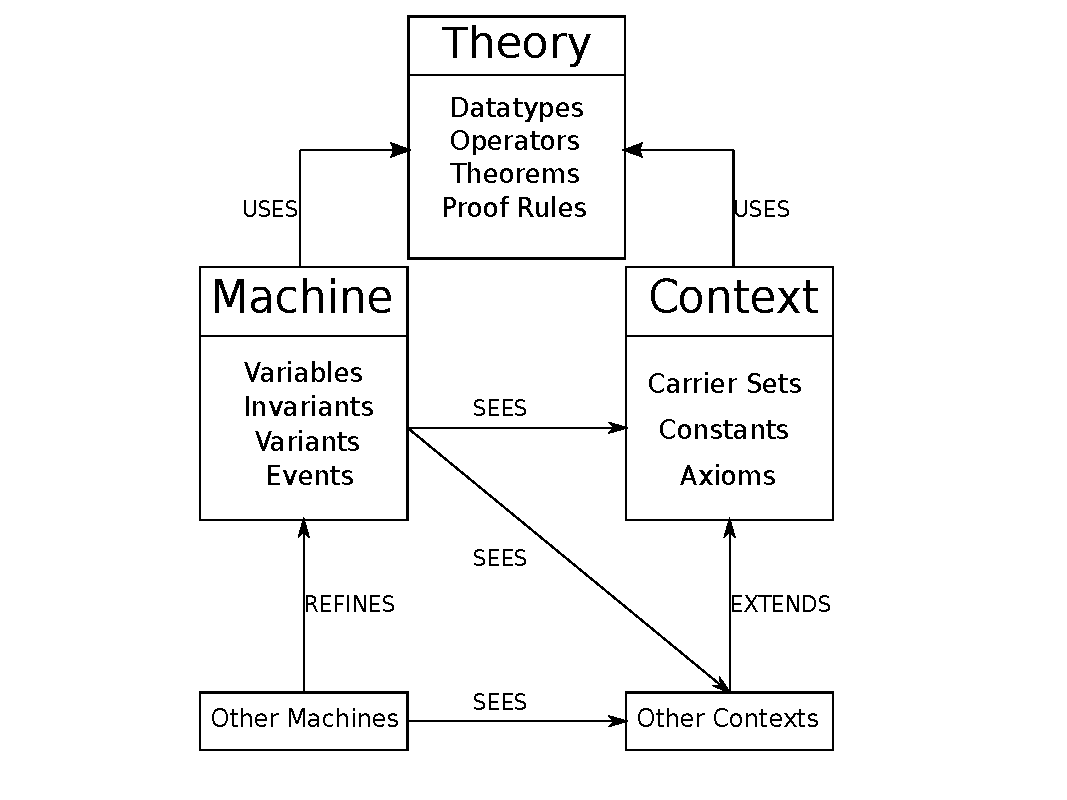
\includegraphics[scale=0.4]{NewComponents}
		\end{figure}
	\end{frame}
	\begin{frame}
		\frametitle{The Theory Component}
		\begin{itemize}
			\item Theories are polymorphic on the type parameters which they define.
			\item A type parameter is a set just like a carrier set in a context.
			\item The only assumption is that it is not empty.
			\item A type parameter can be instantiated with any type.
			\item Potential type instantiation for a type parameter $T$:
				\begin{itemize}
					\item $\mathbb{Z}$
					\item $\pow(\mathbb{Z} \cprod BOOL)$
					\item $TEMP \cprod (\mathbb{Z} \rel JOB)$ where $TEMP$ and $JOB$ are carrier sets.
				\end{itemize}
				\begin{center}
					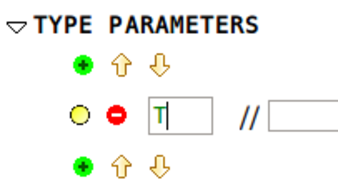
\includegraphics[scale=0.5]{TypeParameter}
				\end{center}
		\end{itemize}
	\end{frame}
\subsection{New Operators}
	\begin{frame}
		\frametitle{The Theory Component $\rightarrow$ Adding New Operators}
		A new Event-B polymorphic operator can be defined by providing the following information in the Theory UI:

~

		\begin{enumerate}
			\item \textit{Parser Information}: this includes the syntax, the notation (infix or prefix), and the syntactic class (term or formula).

~

			\item \textit{Type Checker Information}: this includes the types of the child arguments, and the resultant type if the operator is a term operator.

~
			\item \textit{Prover Information}: this includes the well-definedness of the operator as well as its definition which may be used to reason about it.
		\end{enumerate}
	\end{frame}
	\begin{frame}
		\frametitle{The Theory Component $\rightarrow$ Adding New Operators}
		Parser information includes:

~

		\begin{enumerate}
			\item The syntax symbol, which must be distinct from any previously recognised symbol.

~
			\item The notation: We currently support infix and prefix.

~
			\item The syntactic class: such as,
				\begin{itemize}
					\item an expression operator (like $card$) or,
					\item a predicate operator (like $finite$).
				\end{itemize}
		\end{enumerate}
	\end{frame}
	\begin{frame}
		\frametitle{The Theory Component $\rightarrow$ Adding New Operators}
		Type checker information includes:

~

		\begin{enumerate}
			\item The type of any child arguments of the operator.
				\begin{itemize}
					\item The type of the only child argument of $card$ is a power set of any type $\pow(T)$.

~

				\end{itemize}
			\item The resultant type of the operator \textbf{if} it is an expression operator.
				\begin{itemize}
					\item The resultant type of $card$ is $\mathbb{Z}$.
				\end{itemize}
		\end{enumerate}
		\vspace{5pt}
		\begin{equation*}
			\frac{\textbf{type}(s)~=~\pow(T)}{\textbf{type}(card(s))~=~\mathbb{Z}}~type_{_{card}}
		\end{equation*}
	\end{frame}
	\begin{frame}
		\frametitle{The Theory Component $\rightarrow$ Adding New Operators}
		Prover information includes:

~

		\begin{enumerate}
			\item The definition of the operator.
				\begin{enumerate}
					\item Currently, only direct and recursive definitions are supported.
					\item The definition may only refer to the arguments of the operator and their types.
					\item The definition may be used in proofs as a rewrite.
				\end{enumerate}
~

			\item The well-definedness condition to be used.
				\begin{enumerate}
					\item This will be used (and instantiated) when generating proof obligations.
					\item If no condition is supplied by the user, the well-definedness condition is generated from the direct definition.
				\end{enumerate}

~

			\item Associativity/commutativity properties.
		\end{enumerate}
	\end{frame}
	\begin{frame}
		\frametitle{The Theory Component $\rightarrow$ Proof Obligations}
		Proof obligations are generated to show:

~

		\begin{itemize}
			\item Well-definedness; ensuring that the user-supplied well-definedness condition is stronger than the well-definedness condition of the operator's direct definition.
			\item Commutativity; ensuring that the operator is commutative.
			\item Associativity; ensuring that the operator is associative.
		\end{itemize}

~

		Associativity and commutativity properties are also used to facilitate pattern matching.
	\end{frame}






	\begin{frame}
		\frametitle{The Theory Component $\rightarrow$ Operator Syntax}
		\hrule
		\vspace{3pt}
		\textbf{operator} \textit{name} \\
		$~~~~~~~~$ (\textbf{prefix $\mid$ infix})~~(\textbf{expression $\mid$ predicate})\\
		$~~~~~~~~$ \textbf{args} $x_1\in T_{x_1},..., x_n\in T_{x_n}$\\
		$~~~~~~~~$ \textbf{condition} $P(x_1,...,x_n)$\\
		$~~~~~~~~$ \textbf{definition} $Q(x_1,...,x_n)$\\
		\vspace{3pt}
		\hrule
		\vspace{12pt}
		An Example:
		\vspace{3pt}
		\hrule
		\vspace{3pt}
		\textbf{theory}~~\textit{SeqThy}\\
		\textbf{type parameters}~~$T$\\
		\textbf{operator} \textit{Seq} \textbf{expression} \textbf{prefix}\\
		$~~~~~~~~$ \textbf{args} $a\in \pow(T)$\\
		$~~~~~~~~$ \textbf{condition} $\btrue$\\
		$~~~~~~~~$ \textbf{definition} $\{f,n \cdot f\in 1..n \rightarrow a \mid f\}$
		\vspace{3pt}
		\hrule
	\end{frame}







	\begin{frame}
		\frametitle{The Theory Component $\rightarrow$ A New Sequence}
		\begin{center}
			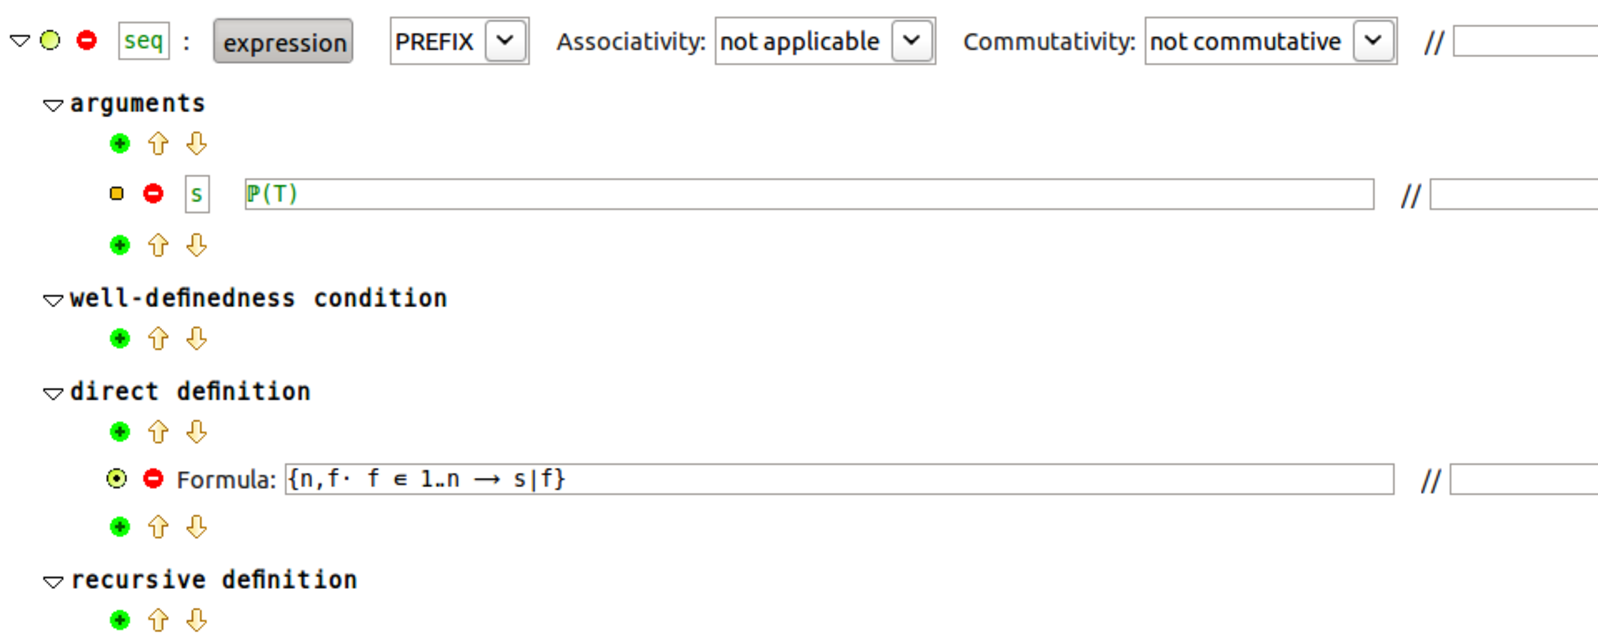
\includegraphics[scale=0.45]{SeqOpDef}
		\end{center}
	\end{frame}
\subsection{Polymorphic Theorems}
	\begin{frame}
		\frametitle{The Theory Component $\rightarrow$ Polymorphic Theorems}
		\begin{itemize}
			\item Conceptually, polymorphic theorems are Event-B predicates that have no free variables.

~

			\item They are polymorphic on the type parameters that occur in them.

~
			\item Sometimes, theorems can be monomorphic if they only refer to the existing types $\mathbb{Z}$ and $BOOL$.
		
~
	\item Examples:
				\begin{enumerate}
					\item $\forall a:\pow(A), b:\pow(A) \cdot a \subseteq b \limp (finite(b) \limp finite(a))$~,
					\item $\forall f:A \rel B, a:\pow(A), b:\pow(B) \cdot f\in a\pfun b \limp (finite(a) \limp finite(f))$~,
					\item $\forall x, y . x * y = 0 \limp (x=0 \lor y=0)$~.
				\end{enumerate}
		\end{itemize}
	\end{frame}






	\begin{frame}
		\frametitle{The Theory Component $\rightarrow$ Polymorphic Theorems}
		\begin{itemize}
			\item Proof obligations generated for theorems:
				\begin{enumerate}
					\item Well-definedness: ensures that the theorem is well-defined.
					\item Validity: ensures that the theorem is valid.
				\end{enumerate}
			\item Similar to Theorems in a Context.
			\item Theorems can be used in proofs by:
				\begin{itemize}
					\item selecting the appropriate theorem in the UI.
					\item providing an appropriate type instantiation, which refers only to types that are recognised by the current sequent.
				\end{itemize}
			\item Once a theorem is appropriately instantiated, it will be added as a selected hypothesis in the current sequent.
		\end{itemize}
	\end{frame}
	\begin{frame}
		\frametitle{The Theory Component $\rightarrow$ Polymorphic Theorems}
		An important use of theorems is the validation of newly added operators. In the case of a sequence operator, we may add the following theorems to ensure the definition captures our understanding:
		\begin{eqnarray*}
			&& \textit{// Seq(a) may be empty} \\
			&&\forall a \in \pow(S) \cdot \emptyset \in Seq(a) ~,\\
			&&~\\
			&&\textit{// array of finite elements}\\
			&&\forall a \in \pow(S) \cdot (\forall s \in \pow(\mathbb{Z}\times S)\cdot s \in Seq(a) \limp finite(s)) ~.
		\end{eqnarray*}
		Needless to say that both these theorems can also be instantiated and used in proofs.
	\end{frame}
	\begin{frame}
		\frametitle{The Theory Component $\rightarrow$ Instantiate in a Proof}
		\begin{center}
			\begin{figure}
				\hfill
				\subfigure[Select a theorem]{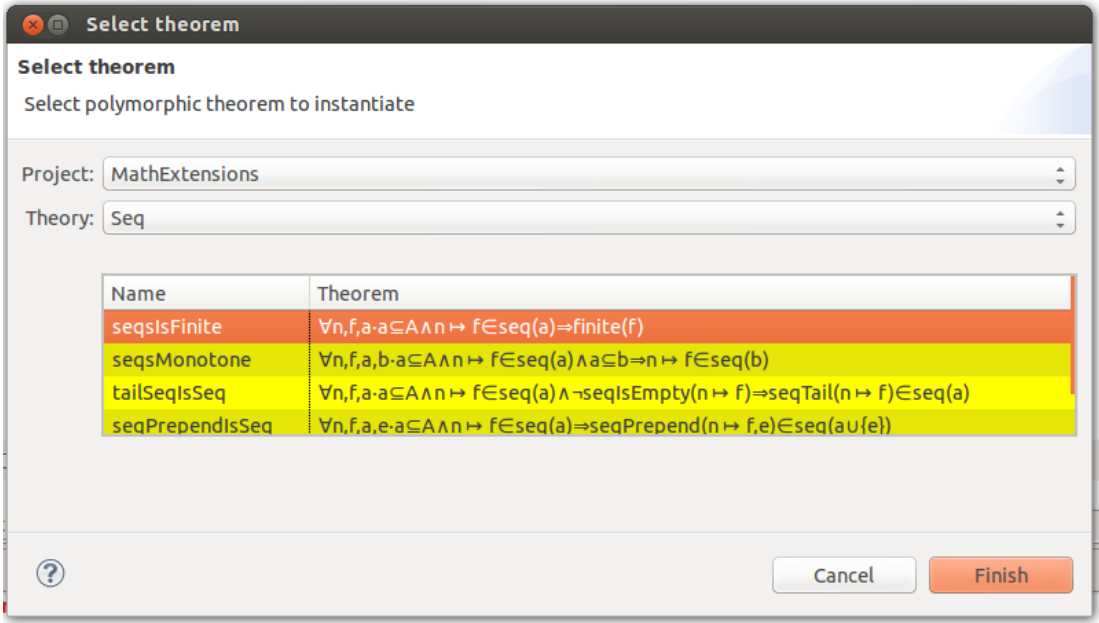
\includegraphics[scale=0.26]{TheoremInst}}
				\hfill
				\subfigure[Instantiate a theorem]{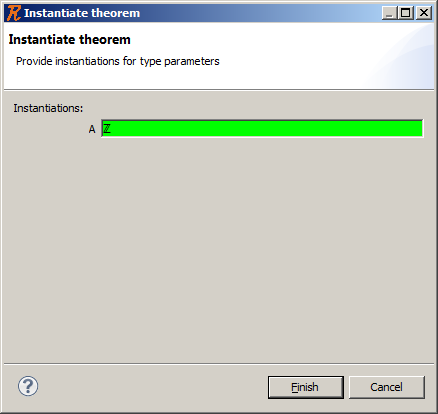
\includegraphics[scale=0.35]{TheoremInst2}}
				\hfill
		\end{figure}
		\end{center}
	\end{frame}
\subsection{Proof Rules}
	\begin{frame}
		\frametitle{The Theory Component $\rightarrow$ Proof Rules}
		\begin{itemize}
			\item The theory components allows the definition of two types of proof rules:
				\begin{enumerate}
					\item \emph{Rewrite rules:}  equalities or equivalences that can be used to rewrite predicates and expressions in sequents.
					\item \emph{Inference rules:} which can be used to discharge, split or add more hypotheses to sequents.
				\end{enumerate}
			\item Proof rules may refer to meta-variables, and type parameters.
			\item Meta-variables are used to facilitate type inference/checking. Each meta-variable has a type.
			\item The rules clause may contain meta-variables, rewrite and inference rules. A theory may contain a number of  blocks.
		\end{itemize}
	\end{frame}
	\begin{frame}
		\frametitle{The Theory Component $\rightarrow$ Proof Rules}
		\begin{center}
			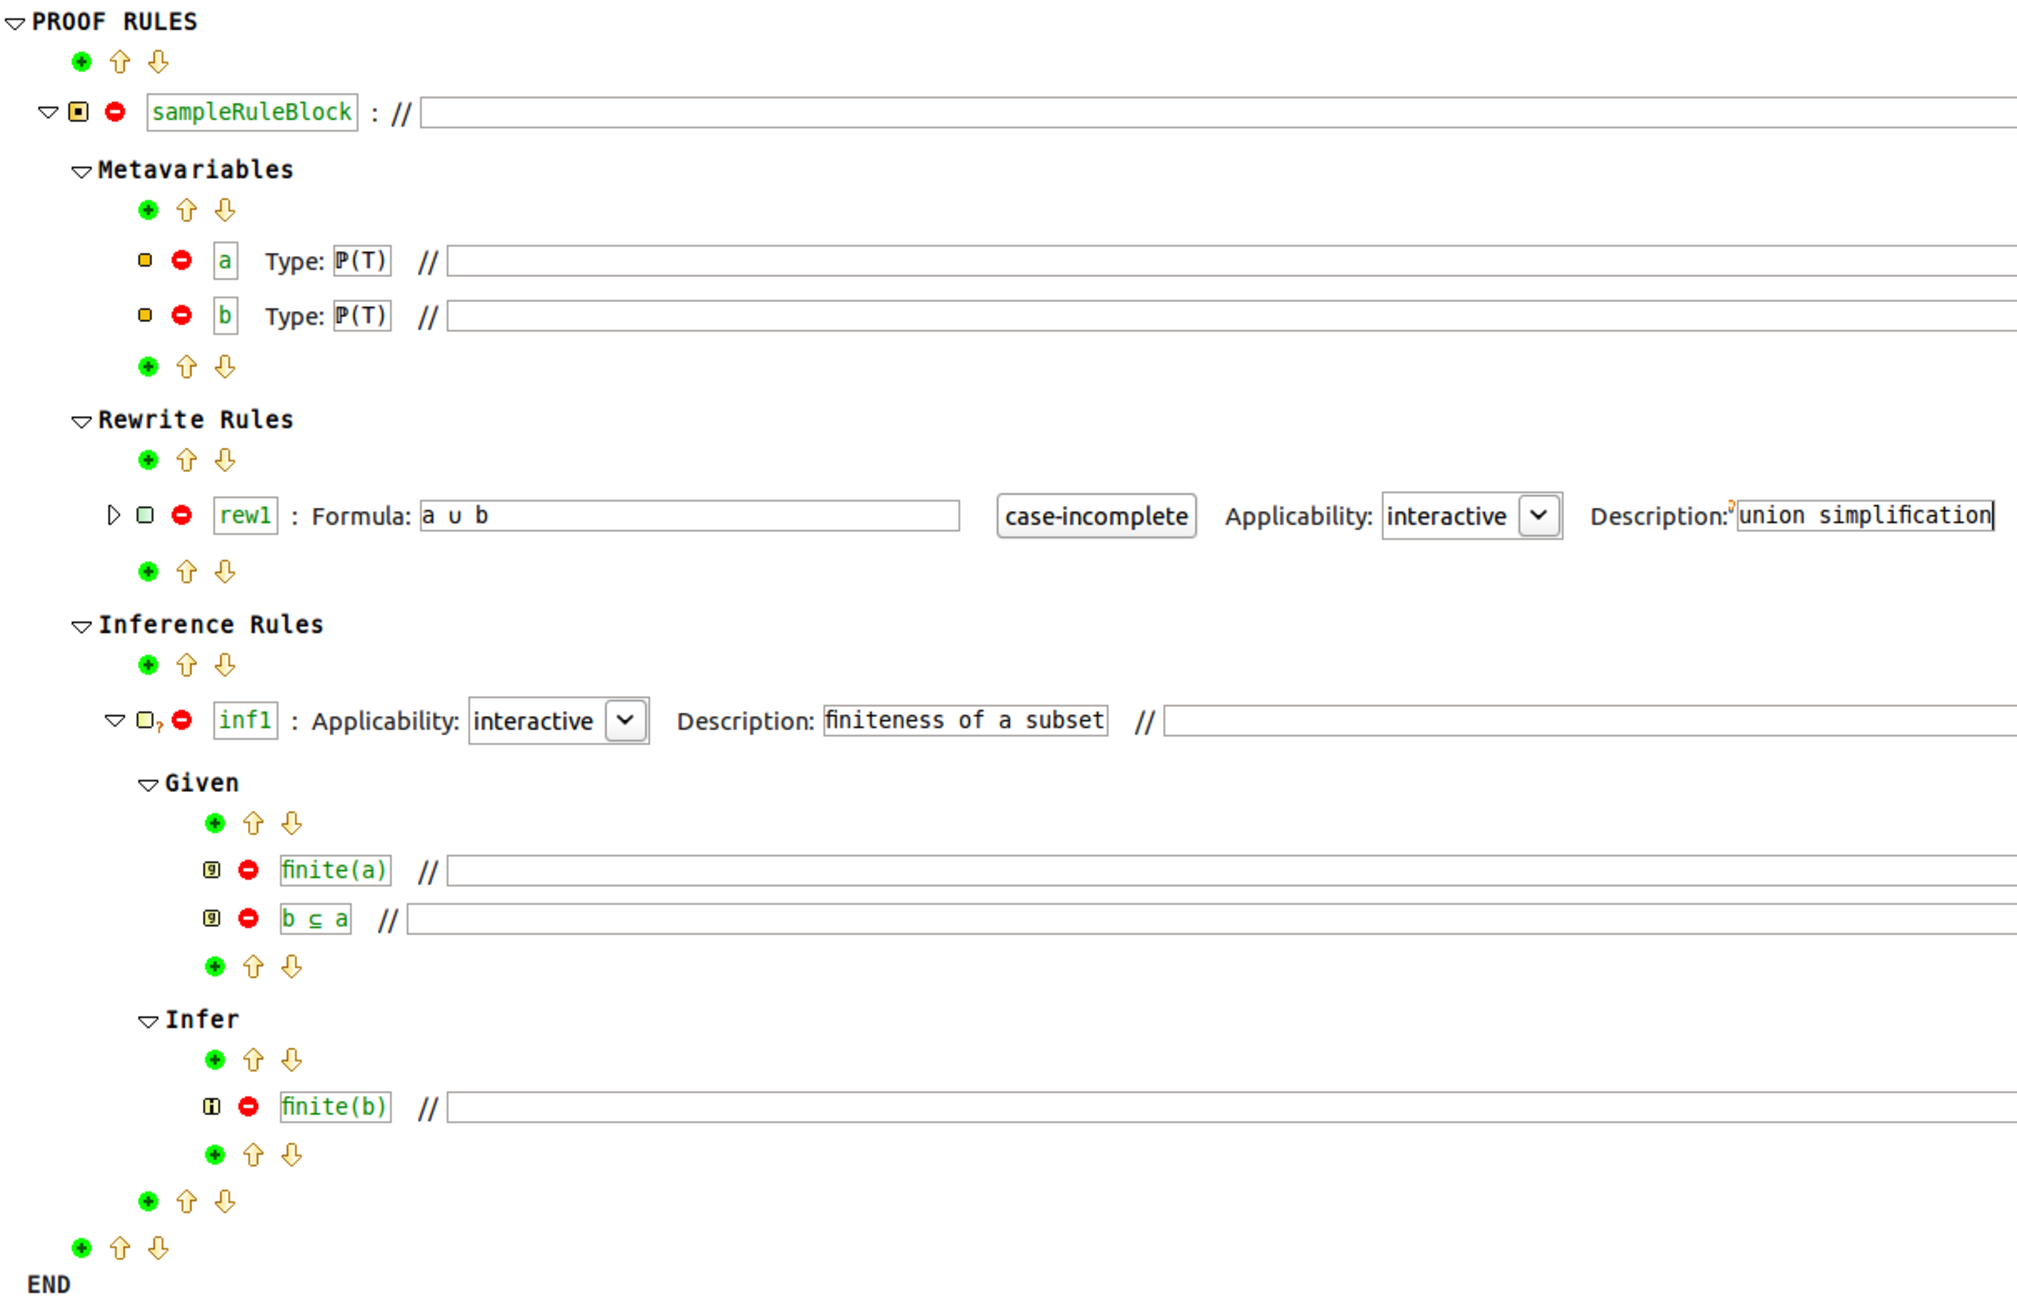
\includegraphics[scale=0.3]{RulesBlock}
		\end{center}
	\end{frame}
\subsubsection{Rewrite Rules}
	\begin{frame}
		\frametitle{The Theory Component $\rightarrow$ Proof Rules $\rightarrow$ Rewrite Rules}
		Rewrite Rules:
		\begin{itemize}
			\item are based on equalities and equivalences.
			\item are polymorphic. But, the plug-in handles instantiation.
			\item can be applied to the goal or hypotheses.
		\end{itemize}


		\begin{itemize}
			\item Examples:
				\begin{enumerate}
					\item $E \in \{F\} ~\defi~ E=F$~,
					\item $union(\pow(S))~\defi~ S$~,
					\item $dom(r^{-1}) ~\defi~ ran(r)$~.
				\end{enumerate}

~

			\item Rewrite rules can be applied automatically or interactively.
			\begin{itemize}
				\item The user decides.
			\end{itemize}
		\end{itemize}
	\end{frame}
	\begin{frame}
		\frametitle{The Theory Component $\rightarrow$ Proof Rules $\rightarrow$ Rewrite Rules}
		\hrule
		\vspace{4pt}
		\textbf{rewrite}~~\textit{name}\\
		$~~~~~~~~~~~$\textbf{[automatic] [interactive] [case complete]}\\
		$~~~~~~~~~~~$\textbf{vars} $x_1:T_{x_1},..., x_n:T_{x_n}$\\
		$~~~~~~~~~~~$\textbf{lhs} $lhs(x_1,..., x_n)$\\
		$~~~~~~~~~~~$\textbf{rhs}\\
		$~~~~~~~~~~~~~~~~$
		\begin{tabular}{|c|c|}
			\hline
				$C_1(x_1,..., x_n)$ & $rhs_1(x_1,..., x_n)$\\\hline
				... & ...\\\hline
				$C_m(x_1,..., x_n)$ & $rhs_m(x_1,..., x_n)$\\
			\hline 
		\end{tabular}
		\vspace{4pt}
		\hrule
		\vspace{3pt}
	\end{frame}
	\begin{frame}
		\frametitle{The Theory Component $\rightarrow$ Proof Rules $\rightarrow$ Rewrite Rules}
		\begin{center}
			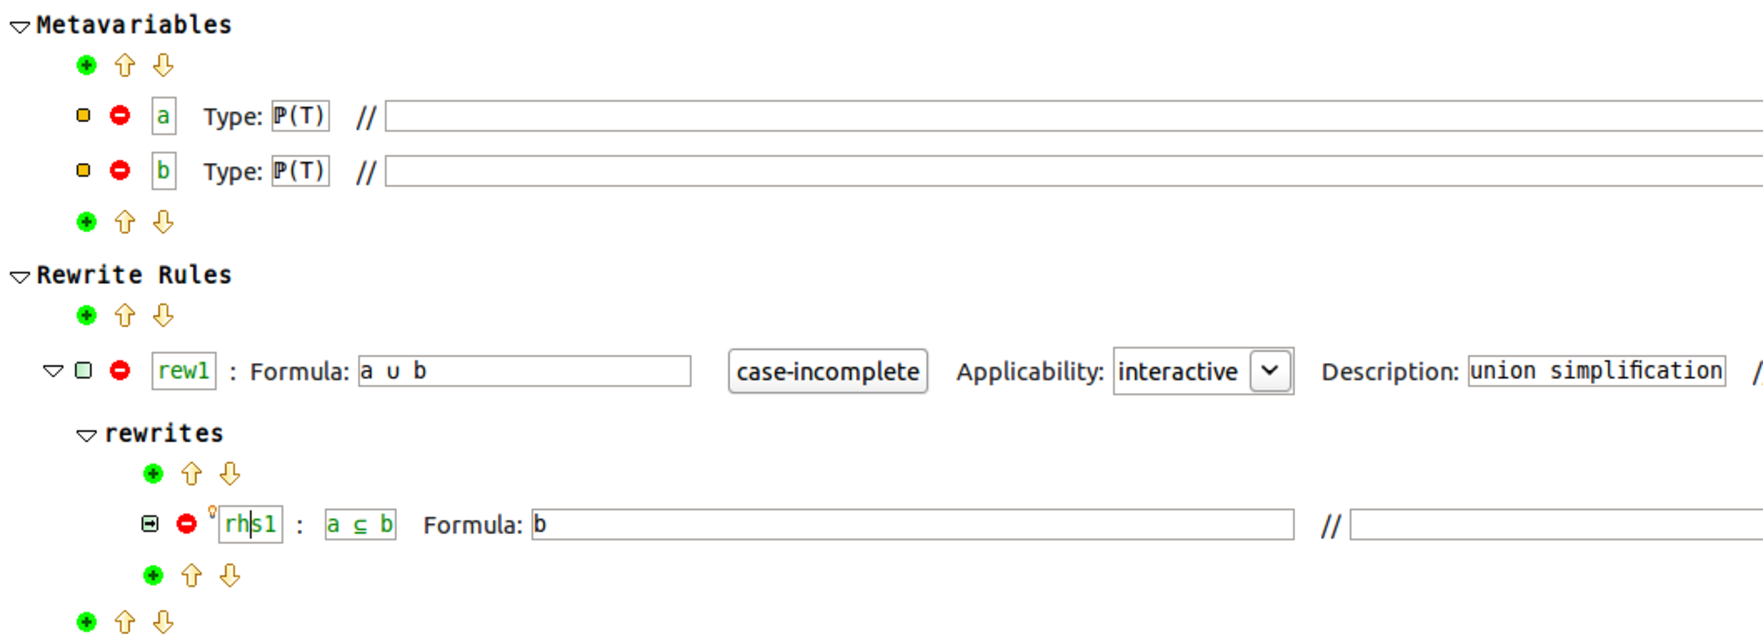
\includegraphics[scale=0.4]{RewRule}
		\end{center}
	\end{frame}
	\begin{frame}
		\frametitle{The Theory Component $\rightarrow$ Proof Rules $\rightarrow$ Rewrite Rules}
		\begin{itemize}
			\item Rewrite rules are generated from operator definitions, e.g.,
				\begin{equation*}
					seq(s)~\defi~\{f,n \cdot f\in 1..n \rightarrow a \mid f\}~.
				\end{equation*}

~

			\item Proof obligations generated for rewrite rules:
				\begin{enumerate}
					\item \emph{Well-definedness preservation:} ensures that well-definedness is not lost when rewriting the left hand side by the right hand side of the rule.
					\item \emph{Equality/Equivalence:} ensures that the rules sides are equal/equivalent under the stipulated conditions.
				\end{enumerate}
		\end{itemize}
		
	\end{frame}
\subsubsection{Inference Rules}
	\begin{frame}
		\frametitle{The Theory Component $\rightarrow$ Proof Rules $\rightarrow$ Inference Rules}
		Inference Rules:
		\begin{itemize}
			\item can be used to discharge, split or add hypotheses to a sequent.

~

			\item are polymorphic. But, the plug-in handles instantiation.

~
			\item can be applied automatically or interactively. 

~
			\item can be applied in a backward as well as forward fashion.

~
			\item as defined in the theory component are a convenient way of applying universally quantified implicative polymorphic theorems.
		\end{itemize}
	\end{frame}
	\begin{frame}
		\frametitle{The Theory Component $\rightarrow$ Proof Rules $\rightarrow$ Inference Rules}
		\hrule
		\vspace{4pt}
		\textbf{inference}~~\textit{name}\\
		$~~~~~~~~~~~$\textbf{[automatic] [interactive]}\\
		$~~~~~~~~~~~$\textbf{vars} $x_1:T_{x_1},..., x_n:T_{x_n}$\\
		$~~~~~~~~~~~$\textbf{given} $H_1,...,H_m$\\
		$~~~~~~~~~~~$\textbf{infer} $I$\\
		\vspace{4pt}
		\hrule
	\end{frame}
	\begin{frame}
		\frametitle{The Theory Component $\rightarrow$ Proof Rules $\rightarrow$ Inference Rules}
		\begin{itemize}
			\item The previous inference rule can be read in two ways:
				\begin{enumerate}
					\item Forward Inference: if you have hypotheses $H_1$,..., $H_m$, you also have hypothesis $I$.
					\item Backward Inference: if you want to prove $I$, it is sufficient to prove each of $H_1$,..., $H_m$.
				\end{enumerate}
			\item The above inference rule can be viewed as a polymorphic theorem:
				\begin{equation}
					\forall \vec{x} \cdot \bigwedge_{i=1}^{m} H_i ~\limp~ I~ \label{polthm}
				\end{equation}
			\item An inference rule is considered sound if its polymorphic theorem (\ref{polthm}) is well-defined and valid.
		\end{itemize}
	\end{frame}
	\begin{frame}
		\frametitle{The Theory Component $\rightarrow$ Proof Rules $\rightarrow$ Inference Rules}
		\begin{center}
			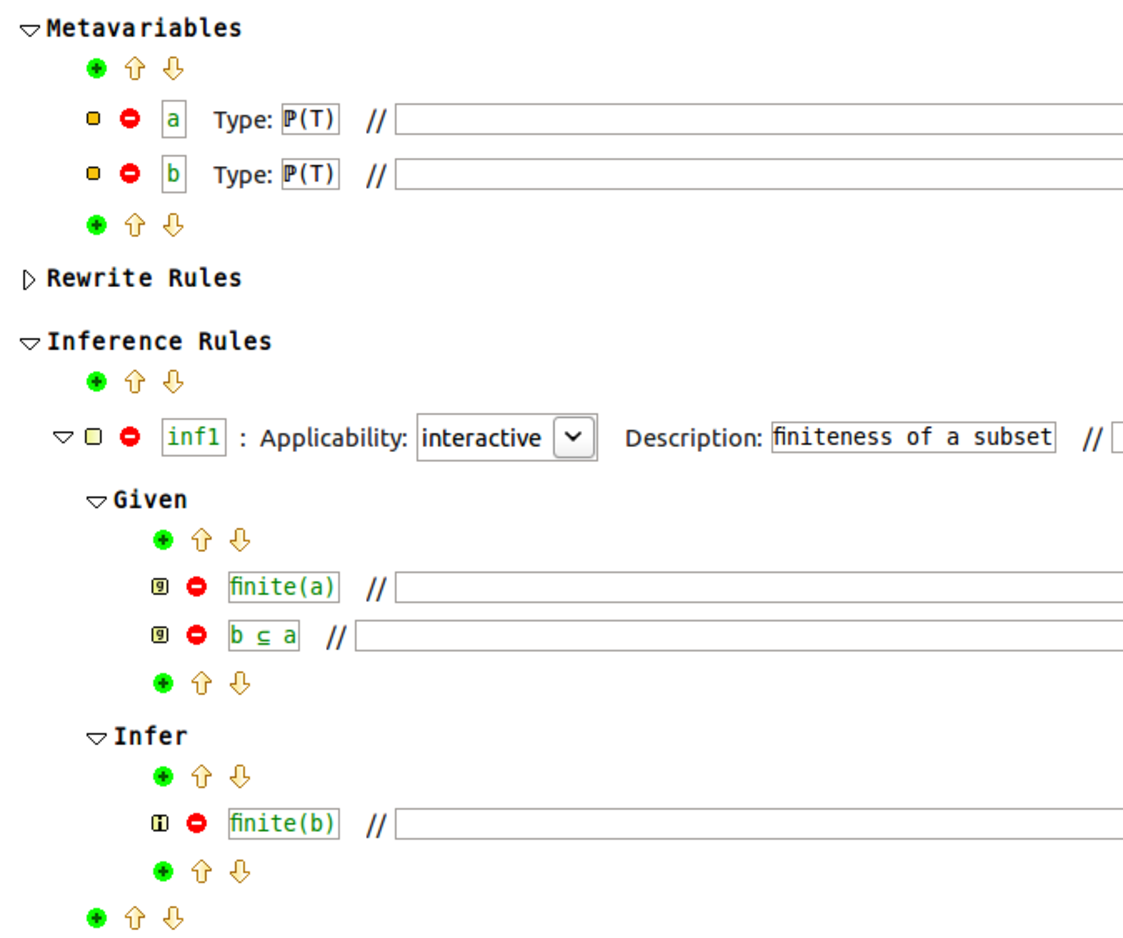
\includegraphics[scale=0.45]{InfRule}
		\end{center}
	\end{frame}
\subsection{Datatypes}
	\begin{frame}
		\frametitle{The Theory Component $\rightarrow$ Datatypes}
		\begin{itemize}
			\item The theory plug-in supports introduction of new datatypes, and recursive functions.
			\item A datatype definition includes a type constructor, element constructors and destructors.
			\item Examples:
				\begin{center}
					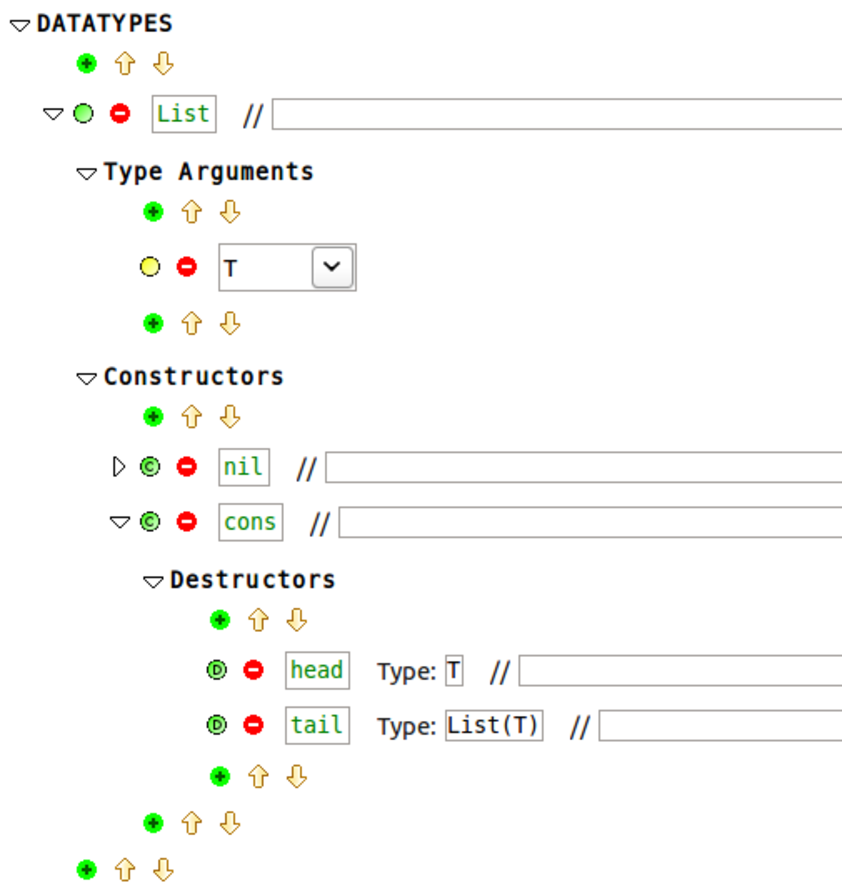
\includegraphics[scale=0.3]{ListDT}
				\end{center}
		\end{itemize}
	\end{frame}
	\begin{frame}
		\frametitle{The Theory Component $\rightarrow$ Datatypes}
		\begin{itemize}
			\item As a result of the above definition, the following expression are legal Event-B expressions:

~

				\begin{enumerate}
					\item $List(T)$

~

					\item $nil$

~
					\item $cons(x, l0)$

~
					\item $head(l)$

~
					\item $tail(l)$
				\end{enumerate}
		\end{itemize}
	\end{frame}
	\begin{frame}
		\frametitle{The Theory Component $\rightarrow$ Datatypes}
		Simple recursive functions can also be defined:
		\begin{center}
			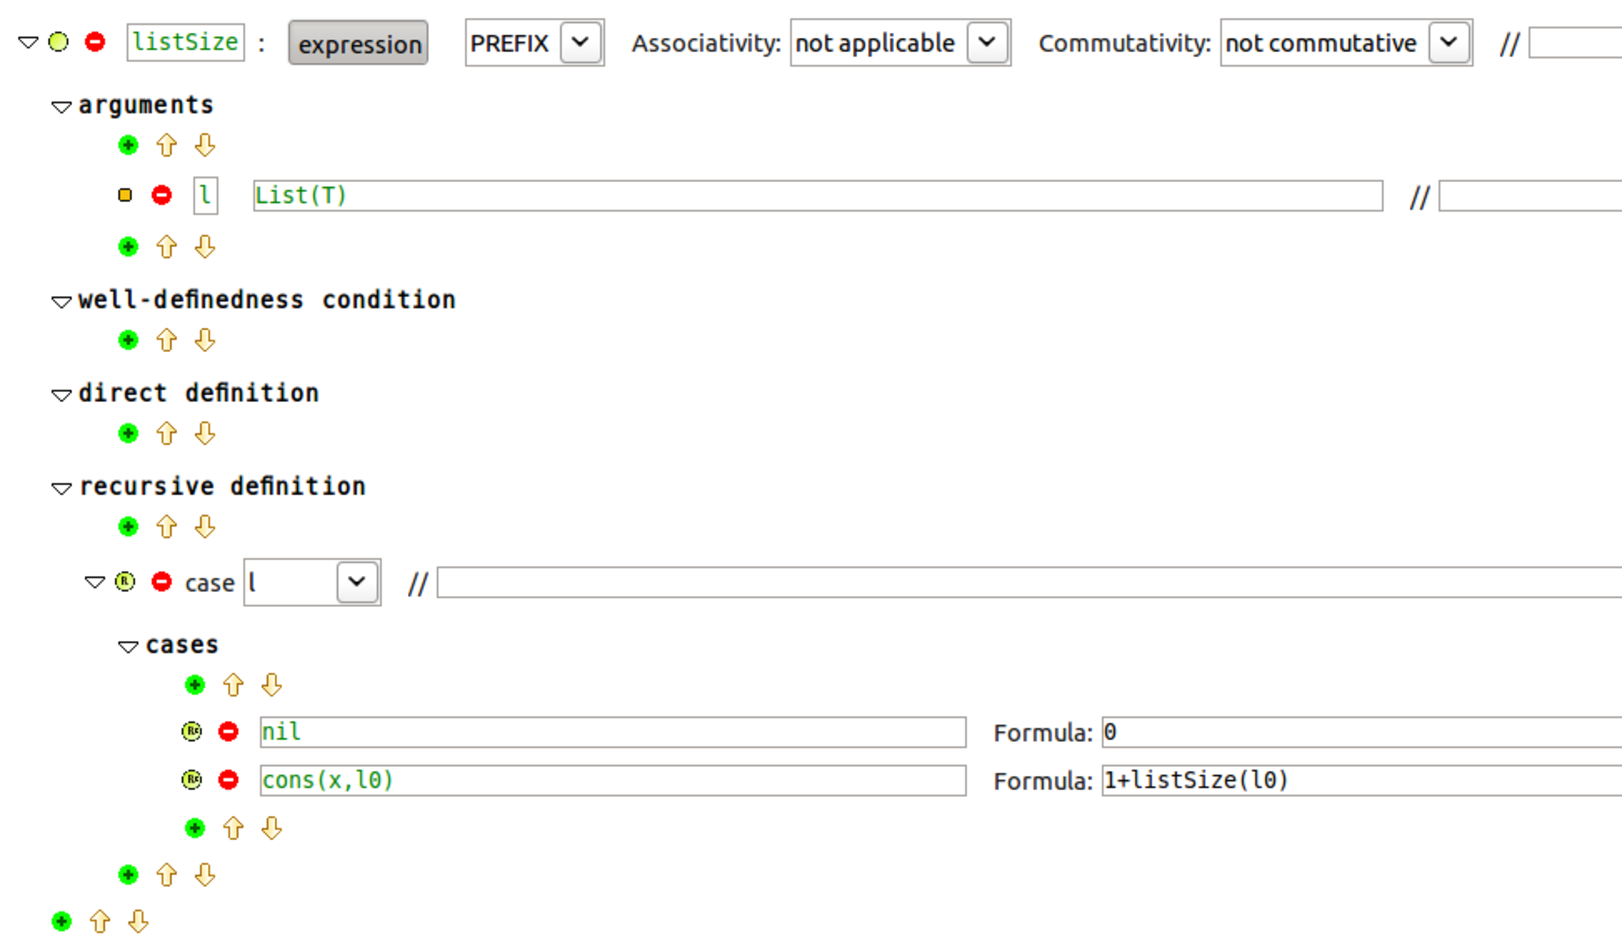
\includegraphics[scale=0.4]{ListSize}
		\end{center}
	\end{frame}
\subsection{Theory Deployment}
	\begin{frame}
		\frametitle{The Theory Component $\rightarrow$ Theory Deployment}
		Deploying the theory:
		\begin{itemize}
			\item is the activity of moving theories from `development stage' to `production stage'.
		\end{itemize}

~

		In the development stage:
		\begin{itemize}
			\item the user develops a hierarchy of theories using the IMPORT directive.
			\item Theories are staticly checked; any proof obligations are generated.
			\item Discharging proof obligations is mandatory before deployment.
		\end{itemize}

~

		After deployment, mathematical and proof extensions are accessible in models and proofs.
	\end{frame}
	\begin{frame}
		\frametitle{The Theory Component $\rightarrow$ Theory Deployment}
		The following tactics are added to the proof interface:
		\begin{enumerate}
			\item \textbf{XD}: (eXpand Definitions) this tactic allows (whenever possible) the rewrite of theory-defined operators occurring in a sequent using their definition.
			\item \textbf{TH}: (polymorphic THeorem) this tactic allows the selection and instantiation of polymorphic theorems.
		\end{enumerate}
		\begin{center}
			
\includegraphics[scale=0.6]{Tactics}
		\end{center}
	\end{frame}
\section{Conclusion}
	\begin{frame}
		\frametitle{Conclusion}
		We have discussed the main features of mathematical extensions using the theory plug-in, including:

~
		\begin{itemize}
 			\item adding new mathematical operators,

~
			\item rewrite rules,

~
			\item inference rules.

~
			\item Polymorphic theorems and their instantation.
		\end{itemize}
	\end{frame}
	\begin{frame}
		\frametitle{Hands-on Session}
		\begin{enumerate}
			\item Develop a theory of sequences.
		\end{enumerate}
		\begin{center}
			
\includegraphics[scale=0.5]{Comp}
		\end{center}
	\end{frame}
\end{document}
